\chapter{Introduzione ad android}
Android è un sistema operativo open-source basato su linux, pensato principalmente per dispositivi mobili, ma anche smart tv e sistemi infotainment per auto.

\begin{figure}[H]
    \centering
    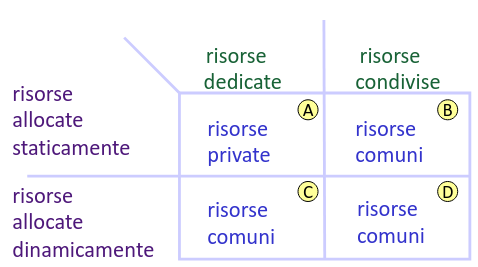
\includegraphics[width=0.7\textwidth]{/home/riccardoob/appunti/sistemi_digitali/images/19.png}
\end{figure}

\subsubsection{Applicazioni}
Layer di più alto livello nello stack android, include applicazione core contenute nel dispostivo di default, le applicazioni sono solitamente scritte in java.

\subsubsection{Framework applicazioni}
Mette a disposizione classi usate per sviluppare le applicazioni, gestisce l'accesso all'hardware fornendo astrazioni per i principali componenti (ad esempio videocamera) e gestisce le interfacce utente e la distribuzione delle risorse.

\subsubsection{Librerie}
Set di librerie che implementano la maggior parte delle funzionalità disponibili nelle librerie core Java.

Anche se le applicazioni Android sono scritte in Java, non vengono eseguite sulla Java Virtual Machine.

\subsubsection{Android runtime}
Librerie core che forniscono la maggiore parte delle funzioni disponibili nelle librerie core Java.

Tra queste è presente la \textbf{Dalvik} virtual machine, una implementazione della JVM specifica per Android, in particolare è scritta per eseguire in modo efficiente diverse istanze della suddetta, ogni applicazione è eseguita nella propria istanza della DVM.


